\documentclass[tikz,border=5pt]{standalone}
\usepackage{tikz}
\usepackage{amsmath}
\usetikzlibrary{arrows.meta}
\definecolor{nebula}{HTML}{6366F1}
\definecolor{spark}{HTML}{14B8A6}
\definecolor{ink}{HTML}{334155}
\begin{document}
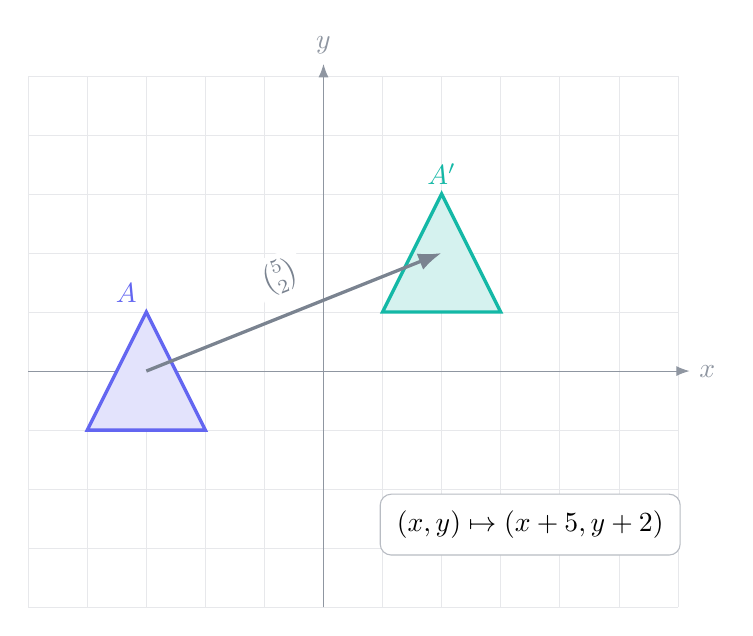
\begin{tikzpicture}[x=.75cm,y=.75cm,font=\sffamily,>=Latex]
  \draw[step=1,very thin,ink!12] (-5,-4) grid (6,5);
  \draw[->,ink!55] (-5,0)--(6.2,0) node[right] {$x$};
  \draw[->,ink!55] (0,-4)--(0,5.2) node[above] {$y$};
  \fill[nebula!18] (-4,-1)--(-2,-1)--(-3,1)--cycle;
  \draw[very thick,nebula] (-4,-1)--(-2,-1)--(-3,1)--cycle;
  \node[nebula,above left] at (-3,1) {$A$};
  \fill[spark!18] (1,1)--(3,1)--(2,3)--cycle;
  \draw[very thick,spark] (1,1)--(3,1)--(2,3)--cycle;
  \node[spark,above] at (2,3) {$A'$};
  \draw[->,very thick,ink!65] (-3,0)--(2,2)
    node[midway,above=5pt,sloped,fill=white,inner sep=2pt] {$\binom{5}{2}$};
  \node[draw=ink!35,rounded corners=4pt,fill=white,inner sep=6pt] at (3.5,-2.6) {$(x,y)\mapsto(x+5,y+2)$};
\end{tikzpicture}
\end{document}
